\documentclass{standalone}
\usepackage{tikz}
\usetikzlibrary{arrows.meta, positioning, fit}

\begin{document}

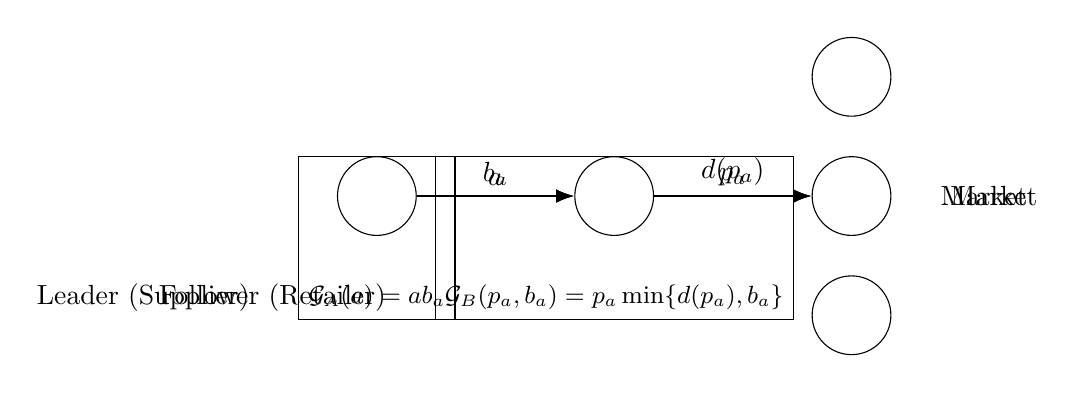
\begin{tikzpicture}[node distance=2cm, >=Latex]

% Define styles for the players
\tikzstyle{player} = [draw, circle, minimum size=1cm]
\tikzstyle{box} = [draw, rectangle, minimum height=1.5cm, minimum width=1.5cm, inner sep=0pt]

% Draw the Leader (Supplier)
\node[player] (leader) {};
\node[below=0.5cm of leader] (leader_label) {\small $\mathcal{G}_A(a) = ab_a$};
\node[fit=(leader)(leader_label), box] {};

\node[left=0.5cm of leader_label] (leader_role) {Leader (Supplier)};

% Draw the Follower (Retailer)
\node[player, right=of leader] (follower) {};
\node[below=0.5cm of follower] (follower_label) {\small $\mathcal{G}_B(p_a, b_a) = p_a \min\{d(p_a), b_a\}$};
\node[fit=(follower)(follower_label), box] {};

\node[left=0.5cm of follower_label] (follower_role) {Follower (Retailer)};

% Draw the Market
\node[player, right=of follower] (market1) {};
\node[player, below=0.5cm of market1] (market2) {};
\node[player, above=0.5cm of market1] (market3) {};
\node[right=0.5cm of market1] (market_role) {Market};

% Arrows and labels
\draw[->, thick] (leader) -- node[above] {$a$} (follower);
\draw[<-, thick] (follower) -- node[above] {$b_a$} (leader);

\draw[->, thick] (follower) -- node[above] {$p_a$} (market1);
\draw[<-, thick] (market1) -- node[above] {$d(p_a)$} (follower);

% Positioning adjustments for the Market
\node[fit=(market1)(market2)(market3), draw=none] (market_box) {};
\node[right=0.5cm of market_box] (market_role) {Market};

\end{tikzpicture}

\end{document}